\documentclass{standalone}
\usepackage{tikz}
\usetikzlibrary{decorations.pathreplacing,decorations.pathmorphing}
\usetikzlibrary{fit,quotes}
\usepackage{yquant, braket}

\begin{document}

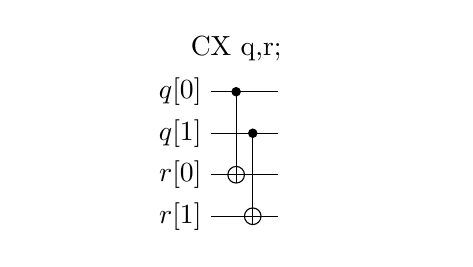
\begin{tikzpicture}[scale=1.000000,x=1pt,y=1pt]
\filldraw[color=white] (0.000000, -7.500000) rectangle (24.000000, 52.500000);
% Drawing wires
% Line 1: q0 W q[0]
\draw[color=black] (0.000000,45.000000) -- (24.000000,45.000000);
\draw[color=black] (0.000000,45.000000) node[left] {$q[0]$};
% Line 2: q1 W q[1]
\draw[color=black] (0.000000,30.000000) -- (24.000000,30.000000);
\draw[color=black] (0.000000,30.000000) node[left] {$q[1]$};
% Line 3: r0 W r[0]
\draw[color=black] (0.000000,15.000000) -- (24.000000,15.000000);
\draw[color=black] (0.000000,15.000000) node[left] {$r[0]$};
% Line 4: r1 W r[1]
\draw[color=black] (0.000000,0.000000) -- (24.000000,0.000000);
\draw[color=black] (0.000000,0.000000) node[left] {$r[1]$};
% Done with wires; drawing gates
% Line 5: q0 +r0		% CX q,r;
\draw (9.000000, 52.500000) node[text width=144pt,above,text centered] {CX q,r;};
\draw (9.000000,45.000000) -- (9.000000,15.000000);
\filldraw (9.000000, 45.000000) circle(1.500000pt);
\begin{scope}
\draw[fill=white] (9.000000, 15.000000) circle(3.000000pt);
\clip (9.000000, 15.000000) circle(3.000000pt);
\draw (6.000000, 15.000000) -- (12.000000, 15.000000);
\draw (9.000000, 12.000000) -- (9.000000, 18.000000);
\end{scope}
% Line 6: q1 +r1
\draw (15.000000,30.000000) -- (15.000000,0.000000);
\filldraw (15.000000, 30.000000) circle(1.500000pt);
\begin{scope}
\draw[fill=white] (15.000000, 0.000000) circle(3.000000pt);
\clip (15.000000, 0.000000) circle(3.000000pt);
\draw (12.000000, 0.000000) -- (18.000000, 0.000000);
\draw (15.000000, -3.000000) -- (15.000000, 3.000000);
\end{scope}
% Done with gates; drawing ending labels
% Done with ending labels; drawing cut lines and comments
% Done with comments
\end{tikzpicture}
\end{document}
